%
% exposit.tex
%    システム制御情報学会  A4版クラスファイル
%    scitrans.cls のサンプル(解説・総説・展望記事のテンプレートファイル)
%
\documentclass[J]{scitrans}
\usepackage{graphicx}
%\usepackage[whole]{bxcjkjatype}
%
%               Usage:  \documentclass[J]{scitrans} (和文の場合)
%                       \documentclass[E]{scitrans} (英文の場合)
%
% 年, 巻, 号 ページの設定
%
\UseRawInputEncoding
\appearyear{1996}
\vol{7}
\numberinvol{13}
\setcounter{page}{1}
\setcounter{volumepage}{1}

\Journal{解説}{『特集名』}{\expositry}      %% 解説の時
%%\Journal{総説}{『特集名』}{\survey}       %% 総説の時
%%\Journal{展望}{『特集名』}{\technicalview}%%  展望の時

%%\Journal{カテゴリ}{}      %% 特集号でない時は, 第2引数を空に

%%\ForSubmission            %% 提出前に一度コメントをはずして
                            %% 英文題目および著者名をご確認ください

\begin{document}

\title{システム制御情報学会スタイルファイルの\\ 使い方\quad
  -- 解説, 展望, 総説の場合--}
\author{鈴木 太郎*}

\etitle{Usage of Style File for Transactions of the Institute of
        Systems, Control and Information Engineers}
\eauthor{Taro {\sc Suzuki}*}
\headingtitle{システム制御情報学会スタイルファイルの使い方}
\headingauthors{システム}

\maketitle

\acceptdate{1995年8月1日}

\address{*}{〇〇大学 工学部}

\keywords{style file, transactions, ISCIE, paper}

%%% つぎの \input を削除し,本文を書き出して下さい.
%-----------------
\section{はじめに}
%-----------------
\label{sec:introduction}

\subsection{概要}

システム制御情報学会クラスファイル{\tt scitrans.cls}は
システム制御情報学会論文誌および会誌「システム/制御/情報」
の記事原稿を作成するための \LaTeX2e クラスファイルです.
{\tt scitrans.cls}は,以下の 9 個のファイル一式として機能します.
これらのファイルを同じディレクトリに置いて下さい.
\begin{itemize}
\item {\tt scitrans.cls}
\item {\tt sci209.sty, scij.sty, scie.sty, scims.sty}
\item {\tt JT1scimc.fd, JT1scigt.fd}
\item {\tt JY1scimc.fd, JY1scigt.fd}
\end{itemize}
このファイル自体が,{\tt scitrans.cls} の
使用例になっていますので,
書き方の参考例としてお使いいただけます.

システム制御情報学会クラスファイル{\tt scitrans.cls}では,
執筆要項に基づいて,文字間のスペースや,改行幅などの設定をしています
(和文の場合,平文では25文字 $\times$ 50行となるようになっています).
また,さまざまなコマンドを用意して,
執筆要項にあった原稿を容易に書けるようにしてあります.

なお,当学会では,{\tt scitrans.cls}を用いて印刷作業を行っていますので,
クラスファイルの内容,設定を無断で変更して作成した原稿を
投稿することはお避けください. 
また,本クラスファイルと同時に使用できるパッケージは
\begin{center}
{\tt graphicx, amsfonts, psfrag}
\end{center}
です.また,{\tt latexsym}が{\tt scitrans.cls}の中で読み込まれています.

以下は,
システム制御情報学会クラスファイルの補足説明です.

\subsection{動作環境}

クラスファイル{\tt scitrans.cls}は,p\TeX{} ver.~p2.1.8
(\TeX{}: ver.~3.14159, Web2C 7.3.1, format: platex 1999.8.10)
を想定して作られています.\LaTeX 209 には対応していません.
{\tt scitrans.cls} に必要な上記のファイルのうち
{\tt scij.sty}には漢字コードが含まれています
(配布しているものはシフトJISおよびEUCコード).
動作環境により漢字コードの扱いが異なりますので,
{\bf 場合によってはコード変換の必要がある}ことにご注意ください.


%-------------------------
\section{和文・英文の区別}
%-------------------------

和文と英文の区別は,\verb+\documentclass+のオプションの指定で行います.
和文の場合は{\tt J}を,英文の場合は{\tt E}を指定します
(和文の場合は\verb+\documentclass+ の\mbox{[ ]}の中に{\tt J}を,
英文の場合は{\tt E}を書きます).
英文の場合,漢字コードを含んだ{\tt scij.sty}を読み込みません.
従って,本文が英文なら日本語に対応していない p\TeX{} でもコンパイルできます.
また,英文の記事でもヘッドラインなどには日本語が用いられますが,
スタイルファイルから漢字コードを排するために,
{\tt E}オプション指定時はヘッドラインなどの日本語の部分は
アスタリスク(****)に置き換えられています
(会誌印刷時には日本語に置き換えられます).

%----------------------------
\section{JIS第1,2水準に含まれない文字を入力する場合}
%
% 原稿中にJISの第1, 2水準に含まれない文字があった場合,その文字の代わり
% に \gaiji{文字の説明} を入力して下さい. もし補助漢字等にあればそのコー
% ドを書いて下さい. ローカルなシステムで作成した外字は使用できません. 
%
原稿中にJISの第1, 2水準に含まれない文字があった場合,
ローカルなシステムで作成した外字は使用できません.
その文字の代わりに \verb%\gaiji{文字の説明}% を入力して下さい. 
もしJIS補助漢字等にあればそのコードを``文字の説明''部分に書いて下さい.  

\noindent 例: \verb%\gaiji{(示韋)}, \gaiji{補助漢字48区70点}%

上記のような記述で作成された原稿には ``\gaiji{文字の説明}''記号が出力されますので,
提出原稿には手書きで正しい漢字を明記してください. 

%-----------------------------------------
\section{プリアンブル}
%-----------------------------------------

会誌の原稿(解説,書評,国際会議の報告など)では \verb+\Journal+ を
プリアンブルで指定してください.
\verb+\Journal+ を指定することによって,
タイトルのレイアウト,図表の番号の付き方などが会誌の書式に準拠したものに
なります
(たとえば会誌では図表番号は,第~1~図,第~1~表などとなります). 

また,英文題目と英文著者名は,本文原稿には現れませんが,
会誌の目次に掲載されますので,これらの情報は会誌原稿の場合でも必要です.
入稿される際にはご確認ください.
\verb+\ForSubmission+を指定すれば,
和文題目,英文題目および英文著者名が,本文の前(0ページ)に出力されま
す.
\verb+\ForSubmission+ のはたらきは,論文誌の場合と異なります.

%---------------
\section{節など}
%---------------
\label{sec:section}

節(section),項(subsection)などの記述は,コマンド 
\verb+\section+, \verb+\subsection+の使用により,
執筆要項に指定されているとおり,
節の表題(大見出し)には2行分をとり,
項以下の表題(中見出し,小見出しなど)は1行分になります.
表題はすべてゴシックになります.

sectionは{\bf 1.},
subsectionは{\bf 1.1},
subsubsectionは{\bf 1.1.1},
paragraphは{\bf (1)},
subparagraphは{\bf (a)}という番号がふられます.
paragraph, subparagraphは直前に空行を入れてください.

例:

\paragraph{パラグラフ}
これは \verb+\paragraph+ の例です.

% \paragraph{空行を入れない場合}
% これは \verb+\paragraph+ の直後に空行を入れない場合です.


%-----------------
\section{定理など}
%-----------------
\label{sec:theorem}

定理などの記述方法に関して,
このクラスファイルでは \verb+\newtheorem+ を使って,
\verb+definition+, \verb+theorem+, \verb+lemma+, \verb+proposition+,
\verb+corollary+, \verb+example+ の環境を定義しています.
また,\verb+\newenvironment+ を使って,
\verb+assumption+, \verb+remark+, \verb+proof+,
\verb+step+ および \verb+condition+ の環境を定義しています.
証明の最後には,□印をつけるようにしています.

以下は,
\verb+theorem+, \verb+proof+, \verb+remark+, \verb+step+,
\verb+condition+ 環境の使用例です.

\begin{theorem}
  \label{theorem:1}
  ここに定理の内容を記述してください.
  系や補題の場合も同様です.
\end{theorem}

\begin{proof}
  ここには定理の証明を記述してください.
  証明の最後には印がつきます.
\end{proof}

\begin{remark}
  \label{remark:1}
  ここには注意を書いてください.
  注意には番号がつくようになっています.
\end{remark}

用意されていない環境を使いたいときには,
次に例を示す \verb+newtheoremenv+, \verb+newparenenv+ が便利です.

\begin{newtheoremenv}{環境がない場合}
  環境が存在しない場合,
  【 】で囲みたいときは newtheoremenv 環境を使ってください.
\end{newtheoremenv}
\begin{newparenenv}{環境がない場合}
  環境が存在しない場合,
  ( )で囲みたいときは newparenenv 環境を使ってください.
\end{newparenenv}

定理などの参照については {\rsec{sec:refer}} で述べます.


%-------------
\section{数式}
%-------------
\label{sec:equation}

{\tt jarticle.cls} では \verb+\eqnarray+環境を使うと,
等号(とは限りませんが)の両側のスペースが広すぎるので,
{\tt scitrans.cls} ではこの間隔を変更しています.
また,{\tt scitrans.cls} では,\verb+\subequations+環境によって,
式番号に\Req{eq:4a}, \Req{eq:4b}などのように副番号をつけることができます.

%%%%%%%%%%%%%%%%%!!!!!!!!!!!!!!!!
{\tt jarticle.cls} では,数式中のギリシャ文字の大文字はローマン体で出
力されますが,
{\tt scitrans.cls} ではこれらの文字は数式イタリック体で
\( \Gamma\Delta\Theta\Lambda\Xi\Pi\Sigma\Upsilon\Phi\Psi\Omega \)
のように出力されます.
数式をボールドで出力するのには \verb+\mbf+ を使います.
ただし,上付きや下付きにするときには,
自動的には大きさが変更されませんので,
意識して \verb+\scriptstyle+ や \verb+\scriptscriptstyle+ を
指定してください.
また,行列の転置記号は \verb+\T+,$\hinf$は \verb+\hinf+ によって出力
することができます.

文中の数式において,単に \verb+$\sum_{k=1}^N$+ とすると,$\sum_{k=1}^N$ 
と出力され,``$k=1$''と``$N$''が $\sum$ の上下につきません.
当学会の書式では,$\displaystyle \sum_{k=1}^N$ とすることになっていますので, 
\verb+$\displaystyle\sum_{k=1}^N$+ のように \verb+\displaystyle+
を用いてください(\verb+\lim+, \verb+\max+, \verb+\min+ なども同様です). 

また,文中に数式を書くとき,``\verb%変数$\zeta$は%'' としたのでは,
``変数$\zeta$は'' のように数式の両側に空白が無く窮屈になってしまう場合
があります.
これを避けるために,\verb+$+$\cdots$\verb+$+の両側に空白を入れて
``変数${}\sqcup$\verb+$\zeta$+${}\sqcup$は'' と記述してください.
これにより,``変数 $\zeta$ は'' のような出力が得られます.

添字については,\verb+{X_a}^b+ または \verb+X_a{}^b+とすると,
${X_a}^b$ のように間延びしてしまいますので,\verb+X_a^b+ として 
$X_a^b$ のように出力してください.

数式モードで,行列や $\displaystyle \int$, $\displaystyle \sum$ 
などの記号を含む数式を括弧で囲む場合には,
\verb+\left(+, \verb+\left\{+, \verb+\right)+, \verb+\right\}+,
あるいは \verb+\Big, \big+ などを用いて括弧の大きさを数式の高さに
合わせてください.

長くて一行におさまらない数式は,見易いところで改行し,
overfullが起こったり,数式と式番号が重なったりしないようにご注意ください.

以下は,数式の例です.
\begin{eqnarray}
        \dot{\mbf{x}}(t) & = & A \mbf{x}(t) + B \mbf{u}(t) 
                               + \sum_{k=1}^N \Gamma_k \mbf{d}k(t)
                \label{eq:1}\\
        \mbf{y}(t) & = & C \mbf{x}(t) + D \mbf{u}(t)
                \label{eq:2}\\
        \mbf{u}(t) & = & F \mbf{x}(t)
                \label{eq:3}
\end{eqnarray}

\begin{subequations}  \label{eq:4}  
  \begin{eqnarray}
    \lefteqn{ 
        \frac{1}{2\pi} \int_{-\infty}^\infty 
        {\rm Tr}\, \{ \mbf{G}\T(-j\omega) \mbf{G}(j\omega) \} \, d\omega 
     }    \hspace*{2zw} \nonumber \\
    & = & 
    \frac{1}{2\pi} \int_{-\infty}^\infty 
    {\rm Tr}\, \{  B\T (-j\omega I -A\T)^{-1}C\T \nonumber \\
    &   & 
    \times C (j\omega I - A)^{-1}B \}\, d\omega 
               \label{eq:4a} \\
    & = & 
    \frac{1}{2\pi j}\int_{-j\infty}^{j\infty} 
    {\rm Tr}\, \left\{ 
    \left[ \begin{array}{c|c} 
       A & B \\ \hline 
       C & 0 \end{array} \right]^\sim  
    \left[ \begin{array}{c|c} 
       A & B \\ \hline 
       C & 0 \end{array} \right]
    \right\} \, ds  
              \label{eq:4b} 
\end{eqnarray}
\end{subequations}

%---------------
\section{図・表}
%---------------
\label{sec:figure and table}

{EPS}ファイルの図を取り込む場合は,{\tt graphicx}パッケージを用い,
%%%(本ファイルのように\verb+\documentclss+の次の行に\verb+\usepackage{graphicx}+と記述)
\verb+\includegraphics+を用いて取り込んで下さい(\rfig{fig:eps}参照).

{\tt scitrans.cls} で定義されている \verb+\tabular+コマンドは,
斜線を入れるなど ISCIE の原稿を出力するための機能が追加されています.
一方,{\tt jarticle.cls}において{\tt jarticle.sty}から拡張された機能は
今のところ実現されていません.

表の作成においては,要素がない部分には,必ず`--'などを入れて
要素がないことを明らかにしてください.
斜線を入れる方法については{\rsec{app:slashbox}}に添付します.
斜線を入れた例を{\rtab{table:slashbox}}に示します.

%
\begin{table}[bt]
	\caption{Example of table ({\tt slashbox.sty})}
	\label{table:slashbox}
	\begin{tabular}{!l!*{2}{c|}c!}\hlinethick
	\backslashbox{部屋}{月/日}
		&\makebox[3em]{5/31} &\makebox[3em]{6/1} &\makebox[3em]{6/2}\\ \hlinethick
		会議室	& --- & --- & --- \\ \hline
		講習会室	& --- & --- & --- \\ \hline
		セミナー室	& --- & --- & --- \\ \hlinethick
	\end{tabular}
\end{table}
%

表の罫線には,太線と細線の2種類を用意してあります.
細線は通常どおりに指定します(縦線は \verb+|+,横線は \verb+\hline+).
太線は,縦線の場合は \verb+!+ を,横線の場合は \verb+\hlinethick+ を
指定してください.
また,本クラスファイルには,{\tt arydshln.sty}も組み込んであるので,
点線も引けるようになっています.
{\rtab{table:1,table:2}}が例となっているので,
参照してください.



%-----------------
\section{参考文献}
%-----------------
\label{sec:bibliography}

参考文献番号を引用箇所の肩につける
場合は \verb+\cite+ を使ってください.
また,「\cite*{foo1}」のように書くときには \verb+\cite*+ を使ってください.
「参考文献」は自動的につきます.
複数の参考文献を肩につけるときには \verb+\cite{foo1,foo2}+,
\verb+\cite{foo2,foo3,foo4}+ のようにしてください.
\mbox{}\cite{foo1,foo2}, \mbox{}\cite{foo2,foo3,foo4} のようになります.
括弧は自動的につくようになっています.


%-------------
\section{参照}
%-------------
\label{sec:refer}

%----------------------------
\begin{figure}[bt]
        \centering
	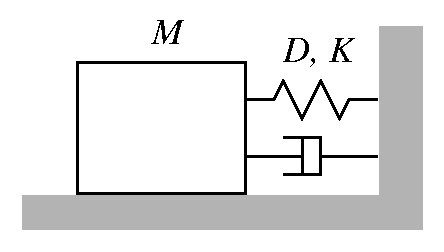
\includegraphics[width=5cm,clip]{tmp.eps}
        \caption{Mass-spring-damper system}
        \label{fig:eps}
\end{figure}
%----------------------------
%
%----------------------------
\setlength{\unitlength}{10mm}
%

\begin{figure}[bt]
        \centering
%
        \begin{picture}(4.5,1)(0,0)
                \thicklines
                \put(0,0.5){\vector(1,0){1.5}}
                \linethickness{1.2pt}
                \put(1.5,0){\framebox(1.5,1){$G(s)$}}
                \thicklines
                \put(3,0.5){\vector(1,0){1.5}}
        \end{picture}
%
        \caption{Plant}
        \label{fig:1}
\end{figure}
%----------------------------
%
%----------------------------
\begin{figure}[bt]
        \centering
%
        \begin{picture}(5.5,2.5)(0,0)
                \thicklines
                \put(0,2){\vector(1,0){0.85}}
                \put(0.7,2.2){\makebox(0,0){$ \scriptstyle + $}}
                \put(1,2){\circle{0.3}}
                \thicklines
                \put(1.15,2){\vector(1,0){0.85}}
                \linethickness{1.2pt}
                \put(2,1.5){\framebox(1.5,1){$G(s)$}}
                \thicklines
                \put(3.5,2){\line(1,0){1}}
                \put(4.5,2){\circle*{0.08}}
                \put(4.5,2){\vector(1,0){1}}
                \put(4.5,2){\line(0,-1){1.5}}
                \put(4.5,0.5){\vector(-1,0){1}}
                \linethickness{1.2pt}
                \put(2,0){\framebox(1.5,1){$H(s)$}}
                \thicklines
                \put(2,0.5){\line(-1,0){1}}
                \put(1,0.5){\vector(0,1){1.35}}
                \put(0.8,1.7){\makebox(0,0){$ \scriptstyle - $}}
        \end{picture}
%
        \caption{Feedback control system}
        \label{fig:2}
\end{figure}

%----------------------------
%
%
%\input{tab01}
%----------------------------
\begin{table}[bt]
        \centering
        \caption{Commands for reference}
        \label{table:1}

        \vspace{0.5\baselineskip}

        \begin{tabular}{!c|l!} \hlinethick
                定義 & \verb+\rdefinition+ \\ \hline
                定理 & \verb+\rtheorem+ \\ \hline
                補題 & \verb+\rlemma+ \\ \hline
                命題 & \verb+\rproposition+ \\ \hline
                系   & \verb+\rcorollary+ \\ \hline
%%              注意 & \verb+\rremark+ \\ \hline
%%              仮定 & \verb+\rassumption+ \\ \hline
                例題 & \verb+\rexample+ \\ \hlinethick
        \end{tabular}
\end{table}
%----------------------------
%
%
%\input{tab02}
%----------------------------
\begin{table}[hbt]
        \centering
        \caption{Commands for reference to equations, figures and tables}
        \label{table:2}

        \vspace{0.5\baselineskip}

        \begin{tabular}{!l|l!} \hlinethick
                式(本文中の番号のみのもの) & \verb+\req+ \\ \hline
                式(付録,副番号付の式など) & \verb+\Req+ \\ \hline
                図 & \verb+\rfig+ \\ \hline
                表 & \verb+\rtab+ \\ \hlinethick
        \end{tabular}
\end{table}
%----------------------------
%

定義,定理などの参照は {\rtab{table:1}} のコマンドを使ってください.
これらのコマンドを使うと,
自動的に「定義」,「定理」などの語が付き,
さらにゴシック体になります(\verb+\rtheorem{theorem:1}+,
\verb+\rremark{remark:1}+ とすれば {\rtheorem{theorem:1}},
{\rremark{remark:1}} のようになります).

また,式,図および表の参照は {\rtab{table:2}} に掲げたコマンドで行えます.
これらのコマンド(\verb+\req{eq:1}+, \verb+\rfig{fig:1}+,
\verb+\rtab{table:1}+ とする)を使うと {\req{eq:1}}, {\rfig{fig:1}},
{\rtab{table:1}} のようになります
(付加される語は \verb+\Transaction+, \verb+\Journal+ の指定によって自動的に
変わります).
複数の式の参照は \verb+\req{eq:1,eq:2}+,
\verb+\req{eq:1,eq:2,eq:3}+ のように
してください
({\req{eq:1,eq:2}},
{\req{eq:1,eq:2,eq:3}} となります).
図表を参照する場合は,
\verb+{\rfig{fig:1,fig:2}}+
のようにしてください
({\rfig{fig:1,fig:2}} となります),

なお,表記の不統一を避けるため,参照には\rtab{table:1,table:2}のコマンドを使い,
\verb+\ref+ は使用しないで下さい.

%-------------
\section{付録}
%-------------

付録の見出しが一つだけの場合は \verb+\section*+ を,
複数ある場合は \verb+\section+ を使ってください.
式番は,付録が複数ある場合でも付録内の通し番号で(A1), (A2)のように
書くことになっていますが,
本文と同様,自動的にそのようになります(\rsec{sec:app}参照).
また,参照する場合は,\verb+{\Req{eq:app1}}+ とすれば
自動的に {\Req{eq:app1}} のようになります.
ただし,
このコマンドは複数の式の参照には対応していないので,
一つずつ参照を行ってください.
%%(本文中の式でも,複数参照する必要がない場合は使えます)


%-----------------
\section{著者略歴}
%-----------------
\label{subsec:aautobiography}

まず,著者略歴を書く位置に \verb+\chosharyakureki+ と書いてください.
つぎに \verb+\authorbiography{+ 著者名 \verb+}+ \verb+{+ ふりがな \verb+}+
\verb+{+ 会員種別 \verb+}+ \verb+{+ 略歴 \verb+}+ の形で
それぞれの要素を書いてください.
著者名とふりがなは5文字どりで次のように書いてください.

\verb+{+ 制,御, ,太,郎 \verb+}+ \verb+{+ せい,ぎょ,,た,ろう \verb+}+

\verb+{+ 情,報, , ,学 \verb+}+ \verb+{+ じょう,ほう,,,まなぶ \verb+}+

また,外国人の場合には次のように姓には \verb+\surname+ を
付けた形で書いてください.ふりがなは必ずしも付ける必要はありません.


\verb+{+Tom,${}\sqcup$,\verb+\surname+${}\sqcup$Cruse\verb+}+ \verb+{+トム,,クルーズ\verb+}+

なお,会誌の記事の場合,対談,座談会,討論,電子メール討論以外の
記事カテゴリーでは,著者略歴は出力されませんが,
これは別ページに掲載しますのでできるだけ著者略歴を入力しておいてください. 

%---------------
\section{その他}
%---------------
\label{sec:miscellaneous}

%-------------------------
\subsection{enumerate環境}
%-------------------------
\label{subsec:enumerate}

enumerate 環境では,番号が(1), (2), $\cdots$ のように
付くようになっています.
これは執筆要項には特に書いてありませんが,
校正段階でこのように合わせているようです.
また,参照するときには式番号と混同するおそれがありますので,
和文の場合は式番号の方には(1)式のように「式」を付けてください
({\rsec{sec:refer}}の \verb+\req+ を使えば自動的につきます).
enumerate 環境の例を示します.
%
\begin{enumerate}
\item これは enumerate 環境の例です.
\item これも enumerate 環境の例です.
\end{enumerate}
%


%----------------
\subsection{脚注}
%----------------
\label{subsec:footnote}

脚注記号は,$1,\ 2,\ \cdots$ の順に
付くようになっています%
\footnote{
  ここが脚注になります.
}%
.
学会誌上では各ページごとにリセットされますので,
それに合わせるために,
{\tt footnpag.sty} を 本クラスファイル中に加えています.

%-----------------------
\subsection{コメントアウト}
%-----------------------
\label{subsec:comment}

大きな範囲をコメントアウトする場合にはコマンド
\verb+\isciecomment+ が便利です.
\verb+\isciecomment{+ $\cdots$ \verb+}+ とすると,
$\cdots$ の部分が出力されなくなります.
%
\isciecomment{
  この部分は出力されません.
}
%

%-----------------
\subsection{括弧,句読点,区切り記号など} 
%-----------------
\label{subsec:punctuation}

日本語\LaTeX は,全角文字と半角文字を区別します.
括弧,句読点(コンマ,ピリオド),区切り記号(コロン,セミコロン)
などは,原則として,和文中では全角文字,英文および数式に対しては
半角文字を用います(もちろん,英文,数式のアルファベットは半角文字です).

また,半角文字の場合,句読点および区切り記号の前にはスペースを入れないで,
後に(半角の)スペースを入れます.

英文に対して\LaTeX は,小文字の後の``ピリオド+スペース''を文末と判断
するようにできています.
そのため,小文字で終わる略語に対しては注意が必要です.
たとえば,単に \verb+Dr.+$\sqcup$\verb+Sato+ としたのでは
Dr.のあとのスペースが大き過ぎます.
これを避けるには,\verb+Dr.~Sato+または\verb+Dr.\+$\sqcup$\verb+Sato+
というように,適当な大きさのスペースをピリオドの後に明示してやります.

%-----------------
\subsection{ハイフネーション} 
%-----------------
\label{subsec;hyphenation}

\TeX はハイフネーションを自動的に行う機能を持っていますが,
固有名詞とその他の英単語を区別しません.
通常,固有名詞のハイフネーションは行いませんので,
行末に英語の固有名詞がくる場合は
\verb+\hyphenation+コマンドを用いて
ハイフネーションを抑制してください.
たとえば,本文中で \verb+\hyphenation{Riccati}+ とすると,
この指定より後にあらわれる ``{\tt Riccati}'' という単語のハイフネーション
は起こりません.

%-----------------
\subsection{URL の表記}
%-----------------
\label{subsec;url}

URL の表記のために\verb+\url+命令が用意されています.
\verb+\url{http://www.iscie.or.jp/}+により
\url{http://www.iscie.or.jp/}と表示されます.
この例のように,2 行にまたがる場合は \verb+/+ のところで改行が入ります.
また,\verb+\url+は書体を変えませんが,例えばタイプライタ体なら
\verb+{\tt\url{http://www.iscie.or.jp/}}+と書体を指定することで
{\tt\url{http://www.iscie.or.jp/}}のように出力することができます.



%-----------------
\section{おわりに}
%-----------------

このクラスファイルには,
改善を要する点が多数含まれていることと存じますが,
会員諸賢によって,
よりよいクラスファイルが作成されるための足がかりとなれば幸いです.
お気づきの点などございましたら,
ISCIE 事務局まで御連絡いただけると幸いです.

% 謝辞
%------------------
\acknowledgement
%-----------------

謝辞には,\verb+\acknowledgement+コマンドをお使い下さい.

このクラスファイルのもとになったB5版スタイルファイルの作成にあたり,
楠見雄規氏(松下電器),田村直之氏(神戸大学)が作成されました
解説用のスタイルファイル({\tt sciart.sty})の一部,
萩原朋道氏(京都大学)が作成されました
論文誌用のスタイルファイル({\tt jhagienv.sty}, {\tt jhagijnl.sty})の一部,
および
ソフトウエア科学会,計測自動制御学会の論文用スタイルファイルを
利用させていただきました.
ありがとうございました.

\begin{thebibliography}{9}
\bibitem{foo1}
        I.\ S.\ Cie:
        The ISCIE style option;
        {\it ISCIE Journal}, Vol.~0, No.~0, pp.~000--999 (1999)

\bibitem{foo2}
        文献:
        ISCIE スタイルオプション;
        システム/制御/情報,Vol.~00, No.~0, pp.~000--999 (1999)

\bibitem{foo3}
        田中,山田:
        論文題目;雑誌名, Vol.~0, No.~0, pp.~00--99 (1999)

\bibitem{foo4}
        Authors:
        Article title, {\it Book Title} (Editor(s), Ed(s).), Publisher,
        pp.~00--99 (1999)
\end{thebibliography}

%% Appendix
%
\appendix

%---------------------
%%\section*{参照コマンド}  %% 付録が一つだけの場合
\section{参照コマンド}     %% 付録が二つ以上の場合
%---------------------
\label{sec:app}

参照コマンドを {\rtab{table:1}} にあげておきます.
式を書くと
%
\begin{equation}
        u = F x
        \label{eq:app1}
\end{equation}
%
のようになります.

%-------------------------
\section{表の斜線の引き方}
%-------------------------
\label{app:slashbox}

以下の文は,{\tt slashbox.sty}に付属のマニュアルに多少変更を加えたものです.
%========================================================================
% slashbox.tex in Japanese
%   The following lines include Shift-JIS (8-bit) KANJI code in JAPAN.

\bigskip %%このようなスペースを空けるコマンドは入稿時には使用しないでください

\begin{tabular}{!l!*{3}{c!}}\hlinethick
\backslashbox{部屋}{月/日}
&\makebox[3em]{5/31}&\makebox[3em]{6/1}&\makebox[3em]{6/2}\\ \hlinethick
会議室&&&\\ \hline
講習会室&&&\\ \hline
セミナー室&&&\\ \hlinethick 
\end{tabular}

\bigskip %%このようなスペースを空けるコマンドは入稿時には使用しないでください

\noindent
のように使います.
「部屋」や「月/日」の中に改行(\verb+\\+)を含めることもできます.
ただし,別の行の同じ欄にもっと幅の広い項目があると,
斜め線の左右にすき間があいてしまいます.
このときは,

\bigskip %%このようなスペースを空けるコマンドは入稿時には使用しないでください

\begin{tabular}{!l!*{2}{c!}} \hlinethick 
\backslashbox[40mm]{部屋}{月/日}
&\makebox[3em]{5/31}&\makebox[3em]{6/1}\\ \hlinethick 
長い長い名前の会議室&&\\ \hline
講習会室&&\\ \hline
セミナー室&&\\ \hlinethick
\end{tabular}

\bigskip %%このようなスペースを空けるコマンドは入稿時には使用しないでください

\noindent
という風にしてその欄の幅を広げて下さい.
ただし指定した寸法が自然な幅より狭いと無視されます.

\verb+\(back)slashbox+ コマンドは,
標準ではその欄の左右に \verb+\tabcolsep+ の空白が入っていると仮定します.
そのため,\verb+@{}+ 等を使うと斜線の端が欄からはみ出たりします.
そのときは,

\bigskip %%このようなスペースを空けるコマンドは入稿時には使用しないでください.

\begin{tabular}{!@{\ $\bullet$\hspace*{3mm}}l!*{3}{c!}} \hlinethick 
\multicolumn{1}{!@{}l!}{\backslashbox[0pt][l]{部屋}{月/日}}
&\makebox[3em]{5/31}&\makebox[4em]{6/1}&\makebox[3em]{6/2}\\ \hlinethick
会議室&&&\\ \hline
講習会室&&&\\ \hline
セミナー室&&&\\ \hlinethick 
\end{tabular}
\bigskip %%このようなスペースを空けるコマンドは入稿時には使用しないでください

\noindent
のようにします.
\verb+[l]+は「この欄の左には空白が入らないと思え」という指定です.
\verb+[r]+や\verb+[lr]+も同様です.
この指定をする場合は欄の幅指定も必要です(0pt でもよい).


\chosharyakureki

\authorbiography{鈴,木, ,太,郎}{すず,き,,た,ろ,う}{正会員}{%
  19XX年X月××大学大学院工学研究科○○工学専攻△△課程修了.
  同年X月××助手.19XX年X月××となり現在に至る.
  ××の研究に従事.
  ××などの会員.}

%\authorbiography{佐,藤, ,花,子}{さ,とう,,はな,こ}{正会員}{%
%  19XX年X月××大学大学院工学研究科○○工学専攻△△課程修了.
%  同年X月××助手.19XX年X月××となり現在に至る.
%  ××の研究に従事.
%  ××などの会員.}

%\authorbiography{田,中, ,次,郎}{た,なか,,じ,ろう}{正会員}{%
%  19XX年X月××大学大学院工学研究科○○工学専攻△△課程修了.
%  同年X月××助手.19XX年X月××となり現在に至る.
%  ××の研究に従事.
%  ××などの会員.}

\end{document}
%
%% end of exposit.tex
